\documentclass[twoside]{book}

% Packages required by doxygen
\usepackage{fixltx2e}
\usepackage{calc}
\usepackage{doxygen}
\usepackage[export]{adjustbox} % also loads graphicx
\usepackage{graphicx}
\usepackage[utf8]{inputenc}
\usepackage{makeidx}
\usepackage{multicol}
\usepackage{multirow}
\PassOptionsToPackage{warn}{textcomp}
\usepackage{textcomp}
\usepackage[nointegrals]{wasysym}
\usepackage[table]{xcolor}

% Font selection
\usepackage[T1]{fontenc}
\usepackage[scaled=.90]{helvet}
\usepackage{courier}
\usepackage{amssymb}
\usepackage{sectsty}
\renewcommand{\familydefault}{\sfdefault}
\allsectionsfont{%
  \fontseries{bc}\selectfont%
  \color{darkgray}%
}
\renewcommand{\DoxyLabelFont}{%
  \fontseries{bc}\selectfont%
  \color{darkgray}%
}
\newcommand{\+}{\discretionary{\mbox{\scriptsize$\hookleftarrow$}}{}{}}

% Page & text layout
\usepackage{geometry}
\geometry{%
  a4paper,%
  top=2.5cm,%
  bottom=2.5cm,%
  left=2.5cm,%
  right=2.5cm%
}
\tolerance=750
\hfuzz=15pt
\hbadness=750
\setlength{\emergencystretch}{15pt}
\setlength{\parindent}{0cm}
\setlength{\parskip}{3ex plus 2ex minus 2ex}
\makeatletter
\renewcommand{\paragraph}{%
  \@startsection{paragraph}{4}{0ex}{-1.0ex}{1.0ex}{%
    \normalfont\normalsize\bfseries\SS@parafont%
  }%
}
\renewcommand{\subparagraph}{%
  \@startsection{subparagraph}{5}{0ex}{-1.0ex}{1.0ex}{%
    \normalfont\normalsize\bfseries\SS@subparafont%
  }%
}
\makeatother

% Headers & footers
\usepackage{fancyhdr}
\pagestyle{fancyplain}
\fancyhead[LE]{\fancyplain{}{\bfseries\thepage}}
\fancyhead[CE]{\fancyplain{}{}}
\fancyhead[RE]{\fancyplain{}{\bfseries\leftmark}}
\fancyhead[LO]{\fancyplain{}{\bfseries\rightmark}}
\fancyhead[CO]{\fancyplain{}{}}
\fancyhead[RO]{\fancyplain{}{\bfseries\thepage}}
\fancyfoot[LE]{\fancyplain{}{}}
\fancyfoot[CE]{\fancyplain{}{}}
\fancyfoot[RE]{\fancyplain{}{\bfseries\scriptsize Generated by Doxygen }}
\fancyfoot[LO]{\fancyplain{}{\bfseries\scriptsize Generated by Doxygen }}
\fancyfoot[CO]{\fancyplain{}{}}
\fancyfoot[RO]{\fancyplain{}{}}
\renewcommand{\footrulewidth}{0.4pt}
\renewcommand{\chaptermark}[1]{%
  \markboth{#1}{}%
}
\renewcommand{\sectionmark}[1]{%
  \markright{\thesection\ #1}%
}

% Indices & bibliography
\usepackage{natbib}
\usepackage[titles]{tocloft}
\setcounter{tocdepth}{3}
\setcounter{secnumdepth}{5}
\makeindex

% Hyperlinks (required, but should be loaded last)
\usepackage{ifpdf}
\ifpdf
  \usepackage[pdftex,pagebackref=true]{hyperref}
\else
  \usepackage[ps2pdf,pagebackref=true]{hyperref}
\fi
\hypersetup{%
  colorlinks=true,%
  linkcolor=blue,%
  citecolor=blue,%
  unicode%
}

% Custom commands
\newcommand{\clearemptydoublepage}{%
  \newpage{\pagestyle{empty}\cleardoublepage}%
}

\usepackage{caption}
\captionsetup{labelsep=space,justification=centering,font={bf},singlelinecheck=off,skip=4pt,position=top}

%===== C O N T E N T S =====

\begin{document}

% Titlepage & ToC
\hypersetup{pageanchor=false,
             bookmarksnumbered=true,
             pdfencoding=unicode
            }
\pagenumbering{roman}
\begin{titlepage}
\vspace*{7cm}
\begin{center}%
{\Large L\+O53 }\\
\vspace*{1cm}
{\large Generated by Doxygen 1.8.11}\\
\end{center}
\end{titlepage}
\clearemptydoublepage
\tableofcontents
\clearemptydoublepage
\pagenumbering{arabic}
\hypersetup{pageanchor=true}

%--- Begin generated contents ---
\chapter{Hierarchical Index}
\section{Class Hierarchy}
This inheritance list is sorted roughly, but not completely, alphabetically\+:\begin{DoxyCompactList}
\item \contentsline{section}{com.\+servlet.\+utilities.\+Fingerprint}{\pageref{classcom_1_1servlet_1_1utilities_1_1_fingerprint}}{}
\item \contentsline{section}{com.\+servlet.\+utilities.\+Location}{\pageref{classcom_1_1servlet_1_1utilities_1_1_location}}{}
\item \contentsline{section}{com.\+servlet.\+utilities.\+Query\+With\+Context}{\pageref{classcom_1_1servlet_1_1utilities_1_1_query_with_context}}{}
\item \contentsline{section}{com.\+servlet.\+utilities.\+Rssi\+Sample}{\pageref{classcom_1_1servlet_1_1utilities_1_1_rssi_sample}}{}
\item \contentsline{section}{com.\+servlet.\+utilities.\+Url\+Address}{\pageref{enumcom_1_1servlet_1_1utilities_1_1_url_address}}{}
\item Http\+Servlet\begin{DoxyCompactList}
\item \contentsline{section}{com.\+servlet.\+calibration.\+Calibration\+Servlet}{\pageref{classcom_1_1servlet_1_1calibration_1_1_calibration_servlet}}{}
\item \contentsline{section}{com.\+servlet.\+debug.\+Debug\+Servlet}{\pageref{classcom_1_1servlet_1_1debug_1_1_debug_servlet}}{}
\item \contentsline{section}{com.\+servlet.\+positioning.\+Positioning\+Servlet}{\pageref{classcom_1_1servlet_1_1positioning_1_1_positioning_servlet}}{}
\end{DoxyCompactList}
\end{DoxyCompactList}

\chapter{Class Index}
\section{Class List}
Here are the classes, structs, unions and interfaces with brief descriptions\+:\begin{DoxyCompactList}
\item\contentsline{section}{\hyperlink{classjwabo_1_1lo53__project_1_1_calibrate_activity}{jwabo.\+lo53\+\_\+project.\+Calibrate\+Activity} }{\pageref{classjwabo_1_1lo53__project_1_1_calibrate_activity}}{}
\item\contentsline{section}{\hyperlink{classjwabo_1_1lo53__project_1_1_locate_activity}{jwabo.\+lo53\+\_\+project.\+Locate\+Activity} }{\pageref{classjwabo_1_1lo53__project_1_1_locate_activity}}{}
\item\contentsline{section}{\hyperlink{classjwabo_1_1lo53__project_1_1_main_activity}{jwabo.\+lo53\+\_\+project.\+Main\+Activity} }{\pageref{classjwabo_1_1lo53__project_1_1_main_activity}}{}
\item\contentsline{section}{\hyperlink{classjwabo_1_1lo53__project_1_1_settings_activity}{jwabo.\+lo53\+\_\+project.\+Settings\+Activity} }{\pageref{classjwabo_1_1lo53__project_1_1_settings_activity}}{}
\end{DoxyCompactList}

\chapter{Class Documentation}
\hypertarget{classcom_1_1servlet_1_1calibration_1_1_calibration_servlet}{}\section{com.\+servlet.\+calibration.\+Calibration\+Servlet Class Reference}
\label{classcom_1_1servlet_1_1calibration_1_1_calibration_servlet}\index{com.\+servlet.\+calibration.\+Calibration\+Servlet@{com.\+servlet.\+calibration.\+Calibration\+Servlet}}
Inheritance diagram for com.\+servlet.\+calibration.\+Calibration\+Servlet\+:\begin{figure}[H]
\begin{center}
\leavevmode
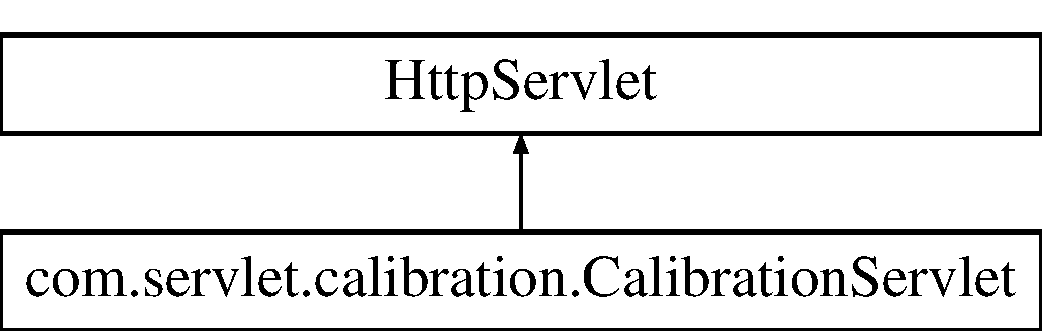
\includegraphics[height=2.000000cm]{classcom_1_1servlet_1_1calibration_1_1_calibration_servlet}
\end{center}
\end{figure}
\subsection*{Public Member Functions}
\begin{DoxyCompactItemize}
\item 
\hyperlink{classcom_1_1servlet_1_1calibration_1_1_calibration_servlet_a97d66eab0eb041965ef4d683ed68fa1d}{Calibration\+Servlet} ()
\end{DoxyCompactItemize}
\subsection*{Protected Member Functions}
\begin{DoxyCompactItemize}
\item 
void \hyperlink{classcom_1_1servlet_1_1calibration_1_1_calibration_servlet_a7f54f8d6e7fe52b09d7268c8ca34ccf3}{do\+Get} (Http\+Servlet\+Request request, Http\+Servlet\+Response response)  throws Servlet\+Exception, I\+O\+Exception 
\item 
void \hyperlink{classcom_1_1servlet_1_1calibration_1_1_calibration_servlet_a62d52c79d84eaa2e4e32bc5d8ceb235e}{do\+Post} (Http\+Servlet\+Request request, Http\+Servlet\+Response response)  throws Servlet\+Exception, I\+O\+Exception 
\end{DoxyCompactItemize}


\subsection{Detailed Description}
Servlet implementation class \hyperlink{classcom_1_1servlet_1_1calibration_1_1_calibration_servlet}{Calibration\+Servlet} 

\subsection{Constructor \& Destructor Documentation}
\index{com\+::servlet\+::calibration\+::\+Calibration\+Servlet@{com\+::servlet\+::calibration\+::\+Calibration\+Servlet}!Calibration\+Servlet@{Calibration\+Servlet}}
\index{Calibration\+Servlet@{Calibration\+Servlet}!com\+::servlet\+::calibration\+::\+Calibration\+Servlet@{com\+::servlet\+::calibration\+::\+Calibration\+Servlet}}
\subsubsection[{\texorpdfstring{Calibration\+Servlet()}{CalibrationServlet()}}]{\setlength{\rightskip}{0pt plus 5cm}com.\+servlet.\+calibration.\+Calibration\+Servlet.\+Calibration\+Servlet (
\begin{DoxyParamCaption}
{}
\end{DoxyParamCaption}
)}\hypertarget{classcom_1_1servlet_1_1calibration_1_1_calibration_servlet_a97d66eab0eb041965ef4d683ed68fa1d}{}\label{classcom_1_1servlet_1_1calibration_1_1_calibration_servlet_a97d66eab0eb041965ef4d683ed68fa1d}
\begin{DoxySeeAlso}{See also}
Http\+Servlet\+::\+Http\+Servlet() Default constructor of a servlet 
\end{DoxySeeAlso}


\subsection{Member Function Documentation}
\index{com\+::servlet\+::calibration\+::\+Calibration\+Servlet@{com\+::servlet\+::calibration\+::\+Calibration\+Servlet}!do\+Get@{do\+Get}}
\index{do\+Get@{do\+Get}!com\+::servlet\+::calibration\+::\+Calibration\+Servlet@{com\+::servlet\+::calibration\+::\+Calibration\+Servlet}}
\subsubsection[{\texorpdfstring{do\+Get(\+Http\+Servlet\+Request request, Http\+Servlet\+Response response)}{doGet(HttpServletRequest request, HttpServletResponse response)}}]{\setlength{\rightskip}{0pt plus 5cm}void com.\+servlet.\+calibration.\+Calibration\+Servlet.\+do\+Get (
\begin{DoxyParamCaption}
\item[{Http\+Servlet\+Request}]{request, }
\item[{Http\+Servlet\+Response}]{response}
\end{DoxyParamCaption}
) throws Servlet\+Exception, I\+O\+Exception\hspace{0.3cm}{\ttfamily [protected]}}\hypertarget{classcom_1_1servlet_1_1calibration_1_1_calibration_servlet_a7f54f8d6e7fe52b09d7268c8ca34ccf3}{}\label{classcom_1_1servlet_1_1calibration_1_1_calibration_servlet_a7f54f8d6e7fe52b09d7268c8ca34ccf3}
\begin{DoxySeeAlso}{See also}
Http\+Servlet\+::do\+Get(\+Http\+Servlet\+Request request, Http\+Servlet\+Response response) 
\end{DoxySeeAlso}
\index{com\+::servlet\+::calibration\+::\+Calibration\+Servlet@{com\+::servlet\+::calibration\+::\+Calibration\+Servlet}!do\+Post@{do\+Post}}
\index{do\+Post@{do\+Post}!com\+::servlet\+::calibration\+::\+Calibration\+Servlet@{com\+::servlet\+::calibration\+::\+Calibration\+Servlet}}
\subsubsection[{\texorpdfstring{do\+Post(\+Http\+Servlet\+Request request, Http\+Servlet\+Response response)}{doPost(HttpServletRequest request, HttpServletResponse response)}}]{\setlength{\rightskip}{0pt plus 5cm}void com.\+servlet.\+calibration.\+Calibration\+Servlet.\+do\+Post (
\begin{DoxyParamCaption}
\item[{Http\+Servlet\+Request}]{request, }
\item[{Http\+Servlet\+Response}]{response}
\end{DoxyParamCaption}
) throws Servlet\+Exception, I\+O\+Exception\hspace{0.3cm}{\ttfamily [protected]}}\hypertarget{classcom_1_1servlet_1_1calibration_1_1_calibration_servlet_a62d52c79d84eaa2e4e32bc5d8ceb235e}{}\label{classcom_1_1servlet_1_1calibration_1_1_calibration_servlet_a62d52c79d84eaa2e4e32bc5d8ceb235e}
\begin{DoxySeeAlso}{See also}
Http\+Servlet\+::do\+Post(\+Http\+Servlet\+Request request, Http\+Servlet\+Response response) When a post request is received, this function is called and process it. Forward request from mobile to waypoints, then retrieve data from waypoints and store into database as calibration data. 
\end{DoxySeeAlso}


The documentation for this class was generated from the following file\+:\begin{DoxyCompactItemize}
\item 
src/com/servlet/calibration/Calibration\+Servlet.\+java\end{DoxyCompactItemize}

\hypertarget{classcom_1_1servlet_1_1debug_1_1_debug_servlet}{}\section{com.\+servlet.\+debug.\+Debug\+Servlet Class Reference}
\label{classcom_1_1servlet_1_1debug_1_1_debug_servlet}\index{com.\+servlet.\+debug.\+Debug\+Servlet@{com.\+servlet.\+debug.\+Debug\+Servlet}}
Inheritance diagram for com.\+servlet.\+debug.\+Debug\+Servlet\+:\begin{figure}[H]
\begin{center}
\leavevmode
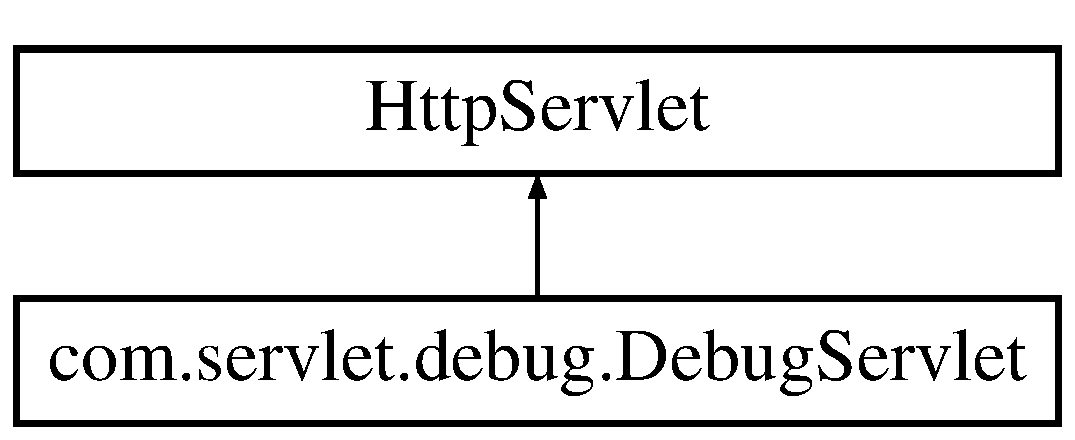
\includegraphics[height=2.000000cm]{classcom_1_1servlet_1_1debug_1_1_debug_servlet}
\end{center}
\end{figure}
\subsection*{Public Member Functions}
\begin{DoxyCompactItemize}
\item 
\hyperlink{classcom_1_1servlet_1_1debug_1_1_debug_servlet_a0059d3aa114ee24bcb93829c9bd81f6d}{Debug\+Servlet} ()
\item 
\hyperlink{classcom_1_1servlet_1_1utilities_1_1_location}{Location} {\bfseries compute\+Location} (Array\+List$<$ \hyperlink{classcom_1_1servlet_1_1utilities_1_1_fingerprint}{Fingerprint} $>$ fingerprints\+Array, \hyperlink{classcom_1_1servlet_1_1utilities_1_1_rssi_sample}{Rssi\+Sample} sample)\hypertarget{classcom_1_1servlet_1_1debug_1_1_debug_servlet_ae8805a36c0afc05ab2e74605c87206af}{}\label{classcom_1_1servlet_1_1debug_1_1_debug_servlet_ae8805a36c0afc05ab2e74605c87206af}

\item 
Array\+List$<$ \hyperlink{classcom_1_1servlet_1_1utilities_1_1_fingerprint}{Fingerprint} $>$ {\bfseries find\+Three\+Nearest\+Locations} (Array\+List$<$ \hyperlink{classcom_1_1servlet_1_1utilities_1_1_fingerprint}{Fingerprint} $>$ fingerprints, \hyperlink{classcom_1_1servlet_1_1utilities_1_1_rssi_sample}{Rssi\+Sample} sample)\hypertarget{classcom_1_1servlet_1_1debug_1_1_debug_servlet_a1cdab7caa7adb17d45ddcd680855e645}{}\label{classcom_1_1servlet_1_1debug_1_1_debug_servlet_a1cdab7caa7adb17d45ddcd680855e645}

\item 
Linked\+Hash\+Map$<$ \hyperlink{classcom_1_1servlet_1_1utilities_1_1_fingerprint}{Fingerprint}, Double $>$ {\bfseries sort\+Hash\+Map\+By\+Values} (Hash\+Map$<$ \hyperlink{classcom_1_1servlet_1_1utilities_1_1_fingerprint}{Fingerprint}, Double $>$ passed\+Map)\hypertarget{classcom_1_1servlet_1_1debug_1_1_debug_servlet_ac79a511aafd41c7932723bcba104370f}{}\label{classcom_1_1servlet_1_1debug_1_1_debug_servlet_ac79a511aafd41c7932723bcba104370f}

\item 
double {\bfseries rssi\+\_\+distance} (\hyperlink{classcom_1_1servlet_1_1utilities_1_1_rssi_sample}{Rssi\+Sample} s1, \hyperlink{classcom_1_1servlet_1_1utilities_1_1_rssi_sample}{Rssi\+Sample} s2)\hypertarget{classcom_1_1servlet_1_1debug_1_1_debug_servlet_a1befae824b1f294a6b631ace389b787a}{}\label{classcom_1_1servlet_1_1debug_1_1_debug_servlet_a1befae824b1f294a6b631ace389b787a}

\end{DoxyCompactItemize}
\subsection*{Protected Member Functions}
\begin{DoxyCompactItemize}
\item 
void \hyperlink{classcom_1_1servlet_1_1debug_1_1_debug_servlet_a3027091a3a446812b8a61e828d9e6197}{do\+Get} (Http\+Servlet\+Request request, Http\+Servlet\+Response response)  throws Servlet\+Exception, I\+O\+Exception 
\item 
void \hyperlink{classcom_1_1servlet_1_1debug_1_1_debug_servlet_a43cf6d116dea0cb2415d5c343e804c14}{do\+Post} (Http\+Servlet\+Request request, Http\+Servlet\+Response response)  throws Servlet\+Exception, I\+O\+Exception 
\end{DoxyCompactItemize}


\subsection{Detailed Description}
Servlet implementation class Positioning\+Servlet 

\subsection{Constructor \& Destructor Documentation}
\index{com\+::servlet\+::debug\+::\+Debug\+Servlet@{com\+::servlet\+::debug\+::\+Debug\+Servlet}!Debug\+Servlet@{Debug\+Servlet}}
\index{Debug\+Servlet@{Debug\+Servlet}!com\+::servlet\+::debug\+::\+Debug\+Servlet@{com\+::servlet\+::debug\+::\+Debug\+Servlet}}
\subsubsection[{\texorpdfstring{Debug\+Servlet()}{DebugServlet()}}]{\setlength{\rightskip}{0pt plus 5cm}com.\+servlet.\+debug.\+Debug\+Servlet.\+Debug\+Servlet (
\begin{DoxyParamCaption}
{}
\end{DoxyParamCaption}
)}\hypertarget{classcom_1_1servlet_1_1debug_1_1_debug_servlet_a0059d3aa114ee24bcb93829c9bd81f6d}{}\label{classcom_1_1servlet_1_1debug_1_1_debug_servlet_a0059d3aa114ee24bcb93829c9bd81f6d}
\begin{DoxySeeAlso}{See also}
Http\+Servlet\+::\+Http\+Servlet() 
\end{DoxySeeAlso}


\subsection{Member Function Documentation}
\index{com\+::servlet\+::debug\+::\+Debug\+Servlet@{com\+::servlet\+::debug\+::\+Debug\+Servlet}!do\+Get@{do\+Get}}
\index{do\+Get@{do\+Get}!com\+::servlet\+::debug\+::\+Debug\+Servlet@{com\+::servlet\+::debug\+::\+Debug\+Servlet}}
\subsubsection[{\texorpdfstring{do\+Get(\+Http\+Servlet\+Request request, Http\+Servlet\+Response response)}{doGet(HttpServletRequest request, HttpServletResponse response)}}]{\setlength{\rightskip}{0pt plus 5cm}void com.\+servlet.\+debug.\+Debug\+Servlet.\+do\+Get (
\begin{DoxyParamCaption}
\item[{Http\+Servlet\+Request}]{request, }
\item[{Http\+Servlet\+Response}]{response}
\end{DoxyParamCaption}
) throws Servlet\+Exception, I\+O\+Exception\hspace{0.3cm}{\ttfamily [protected]}}\hypertarget{classcom_1_1servlet_1_1debug_1_1_debug_servlet_a3027091a3a446812b8a61e828d9e6197}{}\label{classcom_1_1servlet_1_1debug_1_1_debug_servlet_a3027091a3a446812b8a61e828d9e6197}
\begin{DoxySeeAlso}{See also}
Http\+Servlet\+::do\+Get(\+Http\+Servlet\+Request request, Http\+Servlet\+Response response) 
\end{DoxySeeAlso}
\index{com\+::servlet\+::debug\+::\+Debug\+Servlet@{com\+::servlet\+::debug\+::\+Debug\+Servlet}!do\+Post@{do\+Post}}
\index{do\+Post@{do\+Post}!com\+::servlet\+::debug\+::\+Debug\+Servlet@{com\+::servlet\+::debug\+::\+Debug\+Servlet}}
\subsubsection[{\texorpdfstring{do\+Post(\+Http\+Servlet\+Request request, Http\+Servlet\+Response response)}{doPost(HttpServletRequest request, HttpServletResponse response)}}]{\setlength{\rightskip}{0pt plus 5cm}void com.\+servlet.\+debug.\+Debug\+Servlet.\+do\+Post (
\begin{DoxyParamCaption}
\item[{Http\+Servlet\+Request}]{request, }
\item[{Http\+Servlet\+Response}]{response}
\end{DoxyParamCaption}
) throws Servlet\+Exception, I\+O\+Exception\hspace{0.3cm}{\ttfamily [protected]}}\hypertarget{classcom_1_1servlet_1_1debug_1_1_debug_servlet_a43cf6d116dea0cb2415d5c343e804c14}{}\label{classcom_1_1servlet_1_1debug_1_1_debug_servlet_a43cf6d116dea0cb2415d5c343e804c14}
\begin{DoxySeeAlso}{See also}
Http\+Servlet\+::do\+Post(\+Http\+Servlet\+Request request, Http\+Servlet\+Response response) 
\end{DoxySeeAlso}


The documentation for this class was generated from the following file\+:\begin{DoxyCompactItemize}
\item 
src/com/servlet/debug/Debug\+Servlet.\+java\end{DoxyCompactItemize}

\hypertarget{classcom_1_1servlet_1_1utilities_1_1_fingerprint}{}\section{com.\+servlet.\+utilities.\+Fingerprint Class Reference}
\label{classcom_1_1servlet_1_1utilities_1_1_fingerprint}\index{com.\+servlet.\+utilities.\+Fingerprint@{com.\+servlet.\+utilities.\+Fingerprint}}
\subsection*{Public Member Functions}
\begin{DoxyCompactItemize}
\item 
\hyperlink{classcom_1_1servlet_1_1utilities_1_1_location}{Location} {\bfseries get\+Location} ()\hypertarget{classcom_1_1servlet_1_1utilities_1_1_fingerprint_a11cf1858d2d1a4d892cadf7014555693}{}\label{classcom_1_1servlet_1_1utilities_1_1_fingerprint_a11cf1858d2d1a4d892cadf7014555693}

\item 
void {\bfseries set\+Location} (\hyperlink{classcom_1_1servlet_1_1utilities_1_1_location}{Location} location)\hypertarget{classcom_1_1servlet_1_1utilities_1_1_fingerprint_af10716bf3f81917f4e21680823f06a3c}{}\label{classcom_1_1servlet_1_1utilities_1_1_fingerprint_af10716bf3f81917f4e21680823f06a3c}

\item 
\hyperlink{classcom_1_1servlet_1_1utilities_1_1_rssi_sample}{Rssi\+Sample} {\bfseries get\+Measurement} ()\hypertarget{classcom_1_1servlet_1_1utilities_1_1_fingerprint_a6a323bdc32e334e4c4cfd625a7af254d}{}\label{classcom_1_1servlet_1_1utilities_1_1_fingerprint_a6a323bdc32e334e4c4cfd625a7af254d}

\item 
void {\bfseries set\+Measurement} (\hyperlink{classcom_1_1servlet_1_1utilities_1_1_rssi_sample}{Rssi\+Sample} measurement)\hypertarget{classcom_1_1servlet_1_1utilities_1_1_fingerprint_ab56d4888055bf83fe06dc44ff6590e4f}{}\label{classcom_1_1servlet_1_1utilities_1_1_fingerprint_ab56d4888055bf83fe06dc44ff6590e4f}

\end{DoxyCompactItemize}


\subsection{Detailed Description}
Class \hyperlink{classcom_1_1servlet_1_1utilities_1_1_fingerprint}{Fingerprint} 

The documentation for this class was generated from the following file\+:\begin{DoxyCompactItemize}
\item 
src/com/servlet/utilities/Fingerprint.\+java\end{DoxyCompactItemize}

\hypertarget{classcom_1_1servlet_1_1utilities_1_1_location}{}\section{com.\+servlet.\+utilities.\+Location Class Reference}
\label{classcom_1_1servlet_1_1utilities_1_1_location}\index{com.\+servlet.\+utilities.\+Location@{com.\+servlet.\+utilities.\+Location}}
\subsection*{Public Member Functions}
\begin{DoxyCompactItemize}
\item 
\hyperlink{classcom_1_1servlet_1_1utilities_1_1_location_a7ee19224df4270b035459a2d82d4e0cb}{Location} (double x, double y, double z)
\item 
double {\bfseries getX} ()\hypertarget{classcom_1_1servlet_1_1utilities_1_1_location_a5be2885727b60b75f856bab5ba7dbd99}{}\label{classcom_1_1servlet_1_1utilities_1_1_location_a5be2885727b60b75f856bab5ba7dbd99}

\item 
void {\bfseries setX} (double x)\hypertarget{classcom_1_1servlet_1_1utilities_1_1_location_ae06014f28357a9bbf426264e2ea0995e}{}\label{classcom_1_1servlet_1_1utilities_1_1_location_ae06014f28357a9bbf426264e2ea0995e}

\item 
double {\bfseries getY} ()\hypertarget{classcom_1_1servlet_1_1utilities_1_1_location_afffc19a079cbdc9d2cf14ec6083eab79}{}\label{classcom_1_1servlet_1_1utilities_1_1_location_afffc19a079cbdc9d2cf14ec6083eab79}

\item 
void {\bfseries setY} (double y)\hypertarget{classcom_1_1servlet_1_1utilities_1_1_location_acb8e5832a7cc003f2d80b3db6af6d453}{}\label{classcom_1_1servlet_1_1utilities_1_1_location_acb8e5832a7cc003f2d80b3db6af6d453}

\item 
double {\bfseries getZ} ()\hypertarget{classcom_1_1servlet_1_1utilities_1_1_location_ab9d7184b700cf72fb44acb21635d0c89}{}\label{classcom_1_1servlet_1_1utilities_1_1_location_ab9d7184b700cf72fb44acb21635d0c89}

\item 
void {\bfseries setZ} (double z)\hypertarget{classcom_1_1servlet_1_1utilities_1_1_location_a2976c91c6e8269ec0351f1ed686f2bae}{}\label{classcom_1_1servlet_1_1utilities_1_1_location_a2976c91c6e8269ec0351f1ed686f2bae}

\end{DoxyCompactItemize}


\subsection{Detailed Description}
Class \hyperlink{classcom_1_1servlet_1_1utilities_1_1_location}{Location} 

\subsection{Constructor \& Destructor Documentation}
\index{com\+::servlet\+::utilities\+::\+Location@{com\+::servlet\+::utilities\+::\+Location}!Location@{Location}}
\index{Location@{Location}!com\+::servlet\+::utilities\+::\+Location@{com\+::servlet\+::utilities\+::\+Location}}
\subsubsection[{\texorpdfstring{Location(double x, double y, double z)}{Location(double x, double y, double z)}}]{\setlength{\rightskip}{0pt plus 5cm}com.\+servlet.\+utilities.\+Location.\+Location (
\begin{DoxyParamCaption}
\item[{double}]{x, }
\item[{double}]{y, }
\item[{double}]{z}
\end{DoxyParamCaption}
)}\hypertarget{classcom_1_1servlet_1_1utilities_1_1_location_a7ee19224df4270b035459a2d82d4e0cb}{}\label{classcom_1_1servlet_1_1utilities_1_1_location_a7ee19224df4270b035459a2d82d4e0cb}
z coordinate of the location 

The documentation for this class was generated from the following file\+:\begin{DoxyCompactItemize}
\item 
src/com/servlet/utilities/Location.\+java\end{DoxyCompactItemize}

\hypertarget{classcom_1_1servlet_1_1positioning_1_1_positioning_servlet}{}\section{com.\+servlet.\+positioning.\+Positioning\+Servlet Class Reference}
\label{classcom_1_1servlet_1_1positioning_1_1_positioning_servlet}\index{com.\+servlet.\+positioning.\+Positioning\+Servlet@{com.\+servlet.\+positioning.\+Positioning\+Servlet}}
Inheritance diagram for com.\+servlet.\+positioning.\+Positioning\+Servlet\+:\begin{figure}[H]
\begin{center}
\leavevmode
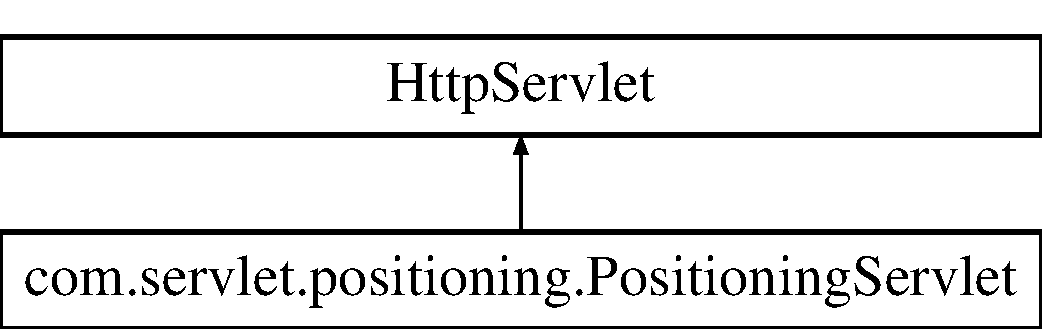
\includegraphics[height=2.000000cm]{classcom_1_1servlet_1_1positioning_1_1_positioning_servlet}
\end{center}
\end{figure}
\subsection*{Public Member Functions}
\begin{DoxyCompactItemize}
\item 
\hyperlink{classcom_1_1servlet_1_1positioning_1_1_positioning_servlet_a9db4dd4f8aedc0ab1cac3e3e176aa8d1}{Positioning\+Servlet} ()
\item 
\hyperlink{classcom_1_1servlet_1_1utilities_1_1_location}{Location} \hyperlink{classcom_1_1servlet_1_1positioning_1_1_positioning_servlet_acfcf3108d3987e97c3987bed9dc7dbbc}{compute\+Location} (Array\+List$<$ \hyperlink{classcom_1_1servlet_1_1utilities_1_1_fingerprint}{Fingerprint} $>$ fingerprints\+Array, \hyperlink{classcom_1_1servlet_1_1utilities_1_1_rssi_sample}{Rssi\+Sample} sample)
\item 
Array\+List$<$ \hyperlink{classcom_1_1servlet_1_1utilities_1_1_fingerprint}{Fingerprint} $>$ \hyperlink{classcom_1_1servlet_1_1positioning_1_1_positioning_servlet_ad8301771d7378366e179f22db3ceca37}{find\+Three\+Nearest\+Locations} (Array\+List$<$ \hyperlink{classcom_1_1servlet_1_1utilities_1_1_fingerprint}{Fingerprint} $>$ fingerprints, \hyperlink{classcom_1_1servlet_1_1utilities_1_1_rssi_sample}{Rssi\+Sample} sample)
\item 
Linked\+Hash\+Map$<$ \hyperlink{classcom_1_1servlet_1_1utilities_1_1_fingerprint}{Fingerprint}, Double $>$ \hyperlink{classcom_1_1servlet_1_1positioning_1_1_positioning_servlet_a39469c71850600fe98758668e72ba179}{sort\+Hash\+Map\+By\+Values} (Hash\+Map$<$ \hyperlink{classcom_1_1servlet_1_1utilities_1_1_fingerprint}{Fingerprint}, Double $>$ passed\+Map)
\item 
double \hyperlink{classcom_1_1servlet_1_1positioning_1_1_positioning_servlet_afdb65734629bb1daec20f1cf445551ab}{rssi\+\_\+distance} (\hyperlink{classcom_1_1servlet_1_1utilities_1_1_rssi_sample}{Rssi\+Sample} s1, \hyperlink{classcom_1_1servlet_1_1utilities_1_1_rssi_sample}{Rssi\+Sample} s2)
\end{DoxyCompactItemize}
\subsection*{Protected Member Functions}
\begin{DoxyCompactItemize}
\item 
void \hyperlink{classcom_1_1servlet_1_1positioning_1_1_positioning_servlet_abe6f2257a6e05ec7c1b2804b8933a633}{do\+Get} (Http\+Servlet\+Request request, Http\+Servlet\+Response response)  throws Servlet\+Exception, I\+O\+Exception 
\item 
void \hyperlink{classcom_1_1servlet_1_1positioning_1_1_positioning_servlet_a82b069325682ed474014b606134163f8}{do\+Post} (Http\+Servlet\+Request request, Http\+Servlet\+Response response)  throws Servlet\+Exception, I\+O\+Exception 
\end{DoxyCompactItemize}


\subsection{Detailed Description}
Servlet \hyperlink{classcom_1_1servlet_1_1positioning_1_1_positioning_servlet}{Positioning\+Servlet} This servlet is used for locating the mobile device. 

\subsection{Constructor \& Destructor Documentation}
\index{com\+::servlet\+::positioning\+::\+Positioning\+Servlet@{com\+::servlet\+::positioning\+::\+Positioning\+Servlet}!Positioning\+Servlet@{Positioning\+Servlet}}
\index{Positioning\+Servlet@{Positioning\+Servlet}!com\+::servlet\+::positioning\+::\+Positioning\+Servlet@{com\+::servlet\+::positioning\+::\+Positioning\+Servlet}}
\subsubsection[{\texorpdfstring{Positioning\+Servlet()}{PositioningServlet()}}]{\setlength{\rightskip}{0pt plus 5cm}com.\+servlet.\+positioning.\+Positioning\+Servlet.\+Positioning\+Servlet (
\begin{DoxyParamCaption}
{}
\end{DoxyParamCaption}
)}\hypertarget{classcom_1_1servlet_1_1positioning_1_1_positioning_servlet_a9db4dd4f8aedc0ab1cac3e3e176aa8d1}{}\label{classcom_1_1servlet_1_1positioning_1_1_positioning_servlet_a9db4dd4f8aedc0ab1cac3e3e176aa8d1}
Map containing M\+AC address of waypoints and the R\+S\+SI values \begin{DoxySeeAlso}{See also}
Http\+Servlet\+::\+Http\+Servlet() Default constructor of a servlet 
\end{DoxySeeAlso}


\subsection{Member Function Documentation}
\index{com\+::servlet\+::positioning\+::\+Positioning\+Servlet@{com\+::servlet\+::positioning\+::\+Positioning\+Servlet}!compute\+Location@{compute\+Location}}
\index{compute\+Location@{compute\+Location}!com\+::servlet\+::positioning\+::\+Positioning\+Servlet@{com\+::servlet\+::positioning\+::\+Positioning\+Servlet}}
\subsubsection[{\texorpdfstring{compute\+Location(\+Array\+List$<$ Fingerprint $>$ fingerprints\+Array, Rssi\+Sample sample)}{computeLocation(ArrayList< Fingerprint > fingerprintsArray, RssiSample sample)}}]{\setlength{\rightskip}{0pt plus 5cm}{\bf Location} com.\+servlet.\+positioning.\+Positioning\+Servlet.\+compute\+Location (
\begin{DoxyParamCaption}
\item[{Array\+List$<$ {\bf Fingerprint} $>$}]{fingerprints\+Array, }
\item[{{\bf Rssi\+Sample}}]{sample}
\end{DoxyParamCaption}
)}\hypertarget{classcom_1_1servlet_1_1positioning_1_1_positioning_servlet_acfcf3108d3987e97c3987bed9dc7dbbc}{}\label{classcom_1_1servlet_1_1positioning_1_1_positioning_servlet_acfcf3108d3987e97c3987bed9dc7dbbc}
Compute the location from distributions of R\+S\+SI values. 
\begin{DoxyParams}{Parameters}
{\em fingerprints\+Array} & an array of fingerprints \\
\hline
{\em sample} & a Rssi\+Sample \\
\hline
\end{DoxyParams}
\begin{DoxyReturn}{Returns}
the location of the mobile device 
\end{DoxyReturn}
\index{com\+::servlet\+::positioning\+::\+Positioning\+Servlet@{com\+::servlet\+::positioning\+::\+Positioning\+Servlet}!do\+Get@{do\+Get}}
\index{do\+Get@{do\+Get}!com\+::servlet\+::positioning\+::\+Positioning\+Servlet@{com\+::servlet\+::positioning\+::\+Positioning\+Servlet}}
\subsubsection[{\texorpdfstring{do\+Get(\+Http\+Servlet\+Request request, Http\+Servlet\+Response response)}{doGet(HttpServletRequest request, HttpServletResponse response)}}]{\setlength{\rightskip}{0pt plus 5cm}void com.\+servlet.\+positioning.\+Positioning\+Servlet.\+do\+Get (
\begin{DoxyParamCaption}
\item[{Http\+Servlet\+Request}]{request, }
\item[{Http\+Servlet\+Response}]{response}
\end{DoxyParamCaption}
) throws Servlet\+Exception, I\+O\+Exception\hspace{0.3cm}{\ttfamily [protected]}}\hypertarget{classcom_1_1servlet_1_1positioning_1_1_positioning_servlet_abe6f2257a6e05ec7c1b2804b8933a633}{}\label{classcom_1_1servlet_1_1positioning_1_1_positioning_servlet_abe6f2257a6e05ec7c1b2804b8933a633}
\begin{DoxySeeAlso}{See also}
Http\+Servlet\+::do\+Get(\+Http\+Servlet\+Request request, Http\+Servlet\+Response response) 
\end{DoxySeeAlso}
\index{com\+::servlet\+::positioning\+::\+Positioning\+Servlet@{com\+::servlet\+::positioning\+::\+Positioning\+Servlet}!do\+Post@{do\+Post}}
\index{do\+Post@{do\+Post}!com\+::servlet\+::positioning\+::\+Positioning\+Servlet@{com\+::servlet\+::positioning\+::\+Positioning\+Servlet}}
\subsubsection[{\texorpdfstring{do\+Post(\+Http\+Servlet\+Request request, Http\+Servlet\+Response response)}{doPost(HttpServletRequest request, HttpServletResponse response)}}]{\setlength{\rightskip}{0pt plus 5cm}void com.\+servlet.\+positioning.\+Positioning\+Servlet.\+do\+Post (
\begin{DoxyParamCaption}
\item[{Http\+Servlet\+Request}]{request, }
\item[{Http\+Servlet\+Response}]{response}
\end{DoxyParamCaption}
) throws Servlet\+Exception, I\+O\+Exception\hspace{0.3cm}{\ttfamily [protected]}}\hypertarget{classcom_1_1servlet_1_1positioning_1_1_positioning_servlet_a82b069325682ed474014b606134163f8}{}\label{classcom_1_1servlet_1_1positioning_1_1_positioning_servlet_a82b069325682ed474014b606134163f8}
\begin{DoxySeeAlso}{See also}
Http\+Servlet\+::do\+Post(\+Http\+Servlet\+Request request, Http\+Servlet\+Response response) When a post request is received, this function is called and process it. Forward request from mobile to waypoints, then retrieve data from waypoints and compute the location and send the location to mobile. 
\end{DoxySeeAlso}
\index{com\+::servlet\+::positioning\+::\+Positioning\+Servlet@{com\+::servlet\+::positioning\+::\+Positioning\+Servlet}!find\+Three\+Nearest\+Locations@{find\+Three\+Nearest\+Locations}}
\index{find\+Three\+Nearest\+Locations@{find\+Three\+Nearest\+Locations}!com\+::servlet\+::positioning\+::\+Positioning\+Servlet@{com\+::servlet\+::positioning\+::\+Positioning\+Servlet}}
\subsubsection[{\texorpdfstring{find\+Three\+Nearest\+Locations(\+Array\+List$<$ Fingerprint $>$ fingerprints, Rssi\+Sample sample)}{findThreeNearestLocations(ArrayList< Fingerprint > fingerprints, RssiSample sample)}}]{\setlength{\rightskip}{0pt plus 5cm}Array\+List$<${\bf Fingerprint}$>$ com.\+servlet.\+positioning.\+Positioning\+Servlet.\+find\+Three\+Nearest\+Locations (
\begin{DoxyParamCaption}
\item[{Array\+List$<$ {\bf Fingerprint} $>$}]{fingerprints, }
\item[{{\bf Rssi\+Sample}}]{sample}
\end{DoxyParamCaption}
)}\hypertarget{classcom_1_1servlet_1_1positioning_1_1_positioning_servlet_ad8301771d7378366e179f22db3ceca37}{}\label{classcom_1_1servlet_1_1positioning_1_1_positioning_servlet_ad8301771d7378366e179f22db3ceca37}
Find the three nearest locations from the current position according to the R\+S\+SI distances 
\begin{DoxyParams}{Parameters}
{\em fingerprints} & an array of fingerprints \\
\hline
{\em sample} & a Rssi\+Sample \\
\hline
\end{DoxyParams}
\begin{DoxyReturn}{Returns}
the location of the mobile device 
\end{DoxyReturn}
\index{com\+::servlet\+::positioning\+::\+Positioning\+Servlet@{com\+::servlet\+::positioning\+::\+Positioning\+Servlet}!rssi\+\_\+distance@{rssi\+\_\+distance}}
\index{rssi\+\_\+distance@{rssi\+\_\+distance}!com\+::servlet\+::positioning\+::\+Positioning\+Servlet@{com\+::servlet\+::positioning\+::\+Positioning\+Servlet}}
\subsubsection[{\texorpdfstring{rssi\+\_\+distance(\+Rssi\+Sample s1, Rssi\+Sample s2)}{rssi_distance(RssiSample s1, RssiSample s2)}}]{\setlength{\rightskip}{0pt plus 5cm}double com.\+servlet.\+positioning.\+Positioning\+Servlet.\+rssi\+\_\+distance (
\begin{DoxyParamCaption}
\item[{{\bf Rssi\+Sample}}]{s1, }
\item[{{\bf Rssi\+Sample}}]{s2}
\end{DoxyParamCaption}
)}\hypertarget{classcom_1_1servlet_1_1positioning_1_1_positioning_servlet_afdb65734629bb1daec20f1cf445551ab}{}\label{classcom_1_1servlet_1_1positioning_1_1_positioning_servlet_afdb65734629bb1daec20f1cf445551ab}
Compute the rssi\+\_\+distance between two Rssi\+Samples 
\begin{DoxyParams}{Parameters}
{\em s1} & a Rssi\+Sample \\
\hline
{\em s2} & a Rssi\+Sample \\
\hline
\end{DoxyParams}
\begin{DoxyReturn}{Returns}
a double value corresponding to the rssi\+\_\+distance 
\end{DoxyReturn}
\index{com\+::servlet\+::positioning\+::\+Positioning\+Servlet@{com\+::servlet\+::positioning\+::\+Positioning\+Servlet}!sort\+Hash\+Map\+By\+Values@{sort\+Hash\+Map\+By\+Values}}
\index{sort\+Hash\+Map\+By\+Values@{sort\+Hash\+Map\+By\+Values}!com\+::servlet\+::positioning\+::\+Positioning\+Servlet@{com\+::servlet\+::positioning\+::\+Positioning\+Servlet}}
\subsubsection[{\texorpdfstring{sort\+Hash\+Map\+By\+Values(\+Hash\+Map$<$ Fingerprint, Double $>$ passed\+Map)}{sortHashMapByValues(HashMap< Fingerprint, Double > passedMap)}}]{\setlength{\rightskip}{0pt plus 5cm}Linked\+Hash\+Map$<${\bf Fingerprint}, Double$>$ com.\+servlet.\+positioning.\+Positioning\+Servlet.\+sort\+Hash\+Map\+By\+Values (
\begin{DoxyParamCaption}
\item[{Hash\+Map$<$ {\bf Fingerprint}, Double $>$}]{passed\+Map}
\end{DoxyParamCaption}
)}\hypertarget{classcom_1_1servlet_1_1positioning_1_1_positioning_servlet_a39469c71850600fe98758668e72ba179}{}\label{classcom_1_1servlet_1_1positioning_1_1_positioning_servlet_a39469c71850600fe98758668e72ba179}
Sort a hash map in decreasing order 
\begin{DoxyParams}{Parameters}
{\em passed\+Map} & a Hash\+Map$<$\+Fingerprint, double$>$ \\
\hline
\end{DoxyParams}
\begin{DoxyReturn}{Returns}
a Linked\+Hash\+Map in the right order 
\end{DoxyReturn}


The documentation for this class was generated from the following file\+:\begin{DoxyCompactItemize}
\item 
src/com/servlet/positioning/Positioning\+Servlet.\+java\end{DoxyCompactItemize}

\hypertarget{classcom_1_1servlet_1_1utilities_1_1_query_with_context}{}\section{com.\+servlet.\+utilities.\+Query\+With\+Context Class Reference}
\label{classcom_1_1servlet_1_1utilities_1_1_query_with_context}\index{com.\+servlet.\+utilities.\+Query\+With\+Context@{com.\+servlet.\+utilities.\+Query\+With\+Context}}
\subsection*{Static Public Member Functions}
\begin{DoxyCompactItemize}
\item 
static void {\bfseries query\+Calibration} (Print\+Writer out)  throws Naming\+Exception \hypertarget{classcom_1_1servlet_1_1utilities_1_1_query_with_context_ae9b1219f8bf7e148ccbbe81d11eece82}{}\label{classcom_1_1servlet_1_1utilities_1_1_query_with_context_ae9b1219f8bf7e148ccbbe81d11eece82}

\item 
static void \hyperlink{classcom_1_1servlet_1_1utilities_1_1_query_with_context_a4addb0131978ad1a87649fbd1deb95e8}{query\+Calibration\+Add\+Location} (String bssid, String x, String y, String z)  throws Naming\+Exception 
\item 
static Array\+List$<$ String $>$ \hyperlink{classcom_1_1servlet_1_1utilities_1_1_query_with_context_a20420a1c44bf30bcd9115964a749f481}{query\+Calibration\+Select\+Waypoints} ()  throws Naming\+Exception 
\item 
static void \hyperlink{classcom_1_1servlet_1_1utilities_1_1_query_with_context_ab7f8d28e27cb314ccfe9e9abe270676a}{query\+Calibration\+Add\+Measurement} (String ypmac, String x, String y, String z, Double value)  throws Naming\+Exception 
\item 
static Array\+List$<$ \hyperlink{classcom_1_1servlet_1_1utilities_1_1_fingerprint}{Fingerprint} $>$ \hyperlink{classcom_1_1servlet_1_1utilities_1_1_query_with_context_a3b7623f0b35b4cfa23a210b4ef73f89a}{query\+Get\+All\+Measurement} ()  throws Naming\+Exception 
\end{DoxyCompactItemize}


\subsection{Member Function Documentation}
\index{com\+::servlet\+::utilities\+::\+Query\+With\+Context@{com\+::servlet\+::utilities\+::\+Query\+With\+Context}!query\+Calibration\+Add\+Location@{query\+Calibration\+Add\+Location}}
\index{query\+Calibration\+Add\+Location@{query\+Calibration\+Add\+Location}!com\+::servlet\+::utilities\+::\+Query\+With\+Context@{com\+::servlet\+::utilities\+::\+Query\+With\+Context}}
\subsubsection[{\texorpdfstring{query\+Calibration\+Add\+Location(\+String bssid, String x, String y, String z)}{queryCalibrationAddLocation(String bssid, String x, String y, String z)}}]{\setlength{\rightskip}{0pt plus 5cm}static void com.\+servlet.\+utilities.\+Query\+With\+Context.\+query\+Calibration\+Add\+Location (
\begin{DoxyParamCaption}
\item[{String}]{bssid, }
\item[{String}]{x, }
\item[{String}]{y, }
\item[{String}]{z}
\end{DoxyParamCaption}
) throws Naming\+Exception\hspace{0.3cm}{\ttfamily [static]}}\hypertarget{classcom_1_1servlet_1_1utilities_1_1_query_with_context_a4addb0131978ad1a87649fbd1deb95e8}{}\label{classcom_1_1servlet_1_1utilities_1_1_query_with_context_a4addb0131978ad1a87649fbd1deb95e8}
Add location into database. 
\begin{DoxyParams}{Parameters}
{\em bssid} & a string \\
\hline
{\em x} & the x coordinate of the location \\
\hline
{\em y} & the y coordinate of the location \\
\hline
{\em z} & the z coordinate of the location \\
\hline
\end{DoxyParams}
\index{com\+::servlet\+::utilities\+::\+Query\+With\+Context@{com\+::servlet\+::utilities\+::\+Query\+With\+Context}!query\+Calibration\+Add\+Measurement@{query\+Calibration\+Add\+Measurement}}
\index{query\+Calibration\+Add\+Measurement@{query\+Calibration\+Add\+Measurement}!com\+::servlet\+::utilities\+::\+Query\+With\+Context@{com\+::servlet\+::utilities\+::\+Query\+With\+Context}}
\subsubsection[{\texorpdfstring{query\+Calibration\+Add\+Measurement(\+String ypmac, String x, String y, String z, Double value)}{queryCalibrationAddMeasurement(String ypmac, String x, String y, String z, Double value)}}]{\setlength{\rightskip}{0pt plus 5cm}static void com.\+servlet.\+utilities.\+Query\+With\+Context.\+query\+Calibration\+Add\+Measurement (
\begin{DoxyParamCaption}
\item[{String}]{ypmac, }
\item[{String}]{x, }
\item[{String}]{y, }
\item[{String}]{z, }
\item[{Double}]{value}
\end{DoxyParamCaption}
) throws Naming\+Exception\hspace{0.3cm}{\ttfamily [static]}}\hypertarget{classcom_1_1servlet_1_1utilities_1_1_query_with_context_ab7f8d28e27cb314ccfe9e9abe270676a}{}\label{classcom_1_1servlet_1_1utilities_1_1_query_with_context_ab7f8d28e27cb314ccfe9e9abe270676a}
Add location into database. 
\begin{DoxyParams}{Parameters}
{\em ypmac} & a string of the M\+AC address of the waypoint \\
\hline
{\em x} & the x coordinate of the location \\
\hline
{\em y} & the y coordinate of the location \\
\hline
{\em z} & the z coordinate of the location \\
\hline
{\em value} & the R\+S\+SI value \\
\hline
\end{DoxyParams}
\index{com\+::servlet\+::utilities\+::\+Query\+With\+Context@{com\+::servlet\+::utilities\+::\+Query\+With\+Context}!query\+Calibration\+Select\+Waypoints@{query\+Calibration\+Select\+Waypoints}}
\index{query\+Calibration\+Select\+Waypoints@{query\+Calibration\+Select\+Waypoints}!com\+::servlet\+::utilities\+::\+Query\+With\+Context@{com\+::servlet\+::utilities\+::\+Query\+With\+Context}}
\subsubsection[{\texorpdfstring{query\+Calibration\+Select\+Waypoints()}{queryCalibrationSelectWaypoints()}}]{\setlength{\rightskip}{0pt plus 5cm}static Array\+List$<$String$>$ com.\+servlet.\+utilities.\+Query\+With\+Context.\+query\+Calibration\+Select\+Waypoints (
\begin{DoxyParamCaption}
{}
\end{DoxyParamCaption}
) throws Naming\+Exception\hspace{0.3cm}{\ttfamily [static]}}\hypertarget{classcom_1_1servlet_1_1utilities_1_1_query_with_context_a20420a1c44bf30bcd9115964a749f481}{}\label{classcom_1_1servlet_1_1utilities_1_1_query_with_context_a20420a1c44bf30bcd9115964a749f481}
Get all the waypoints M\+AC address. \begin{DoxyReturn}{Returns}
an array of all the M\+AC addresses 
\end{DoxyReturn}
\index{com\+::servlet\+::utilities\+::\+Query\+With\+Context@{com\+::servlet\+::utilities\+::\+Query\+With\+Context}!query\+Get\+All\+Measurement@{query\+Get\+All\+Measurement}}
\index{query\+Get\+All\+Measurement@{query\+Get\+All\+Measurement}!com\+::servlet\+::utilities\+::\+Query\+With\+Context@{com\+::servlet\+::utilities\+::\+Query\+With\+Context}}
\subsubsection[{\texorpdfstring{query\+Get\+All\+Measurement()}{queryGetAllMeasurement()}}]{\setlength{\rightskip}{0pt plus 5cm}static Array\+List$<${\bf Fingerprint}$>$ com.\+servlet.\+utilities.\+Query\+With\+Context.\+query\+Get\+All\+Measurement (
\begin{DoxyParamCaption}
{}
\end{DoxyParamCaption}
) throws Naming\+Exception\hspace{0.3cm}{\ttfamily [static]}}\hypertarget{classcom_1_1servlet_1_1utilities_1_1_query_with_context_a3b7623f0b35b4cfa23a210b4ef73f89a}{}\label{classcom_1_1servlet_1_1utilities_1_1_query_with_context_a3b7623f0b35b4cfa23a210b4ef73f89a}
Get all the measurements. \begin{DoxyReturn}{Returns}
an array of all the fingerprints 
\end{DoxyReturn}


The documentation for this class was generated from the following file\+:\begin{DoxyCompactItemize}
\item 
src/com/servlet/utilities/Query\+With\+Context.\+java\end{DoxyCompactItemize}

\hypertarget{classcom_1_1servlet_1_1utilities_1_1_rssi_sample}{}\section{com.\+servlet.\+utilities.\+Rssi\+Sample Class Reference}
\label{classcom_1_1servlet_1_1utilities_1_1_rssi_sample}\index{com.\+servlet.\+utilities.\+Rssi\+Sample@{com.\+servlet.\+utilities.\+Rssi\+Sample}}
\subsection*{Public Member Functions}
\begin{DoxyCompactItemize}
\item 
\hyperlink{classcom_1_1servlet_1_1utilities_1_1_rssi_sample_a8c6bab7c92d6251e21c669d308384f07}{Rssi\+Sample} (Map$<$ String, Double $>$ map\+Gotchas)
\item 
Map$<$ String, Double $>$ {\bfseries get\+Rssi} ()\hypertarget{classcom_1_1servlet_1_1utilities_1_1_rssi_sample_a0cd6954366a535aceaff70a6f6e69000}{}\label{classcom_1_1servlet_1_1utilities_1_1_rssi_sample_a0cd6954366a535aceaff70a6f6e69000}

\item 
void {\bfseries set\+Rssi} (Hash\+Map$<$ String, Double $>$ rssi)\hypertarget{classcom_1_1servlet_1_1utilities_1_1_rssi_sample_a2a1ce4425cd0df01b930d37c20a81e78}{}\label{classcom_1_1servlet_1_1utilities_1_1_rssi_sample_a2a1ce4425cd0df01b930d37c20a81e78}

\end{DoxyCompactItemize}


\subsection{Detailed Description}
Class \hyperlink{classcom_1_1servlet_1_1utilities_1_1_rssi_sample}{Rssi\+Sample} 

\subsection{Constructor \& Destructor Documentation}
\index{com\+::servlet\+::utilities\+::\+Rssi\+Sample@{com\+::servlet\+::utilities\+::\+Rssi\+Sample}!Rssi\+Sample@{Rssi\+Sample}}
\index{Rssi\+Sample@{Rssi\+Sample}!com\+::servlet\+::utilities\+::\+Rssi\+Sample@{com\+::servlet\+::utilities\+::\+Rssi\+Sample}}
\subsubsection[{\texorpdfstring{Rssi\+Sample(\+Map$<$ String, Double $>$ map\+Gotchas)}{RssiSample(Map< String, Double > mapGotchas)}}]{\setlength{\rightskip}{0pt plus 5cm}com.\+servlet.\+utilities.\+Rssi\+Sample.\+Rssi\+Sample (
\begin{DoxyParamCaption}
\item[{Map$<$ String, Double $>$}]{map\+Gotchas}
\end{DoxyParamCaption}
)}\hypertarget{classcom_1_1servlet_1_1utilities_1_1_rssi_sample_a8c6bab7c92d6251e21c669d308384f07}{}\label{classcom_1_1servlet_1_1utilities_1_1_rssi_sample_a8c6bab7c92d6251e21c669d308384f07}
Map containing the M\+AC address of the waypoint and the R\+S\+SI value associated with it 

The documentation for this class was generated from the following file\+:\begin{DoxyCompactItemize}
\item 
src/com/servlet/utilities/Rssi\+Sample.\+java\end{DoxyCompactItemize}

\hypertarget{enumcom_1_1servlet_1_1utilities_1_1_url_address}{}\section{com.\+servlet.\+utilities.\+Url\+Address Enum Reference}
\label{enumcom_1_1servlet_1_1utilities_1_1_url_address}\index{com.\+servlet.\+utilities.\+Url\+Address@{com.\+servlet.\+utilities.\+Url\+Address}}
\subsection*{Public Member Functions}
\begin{DoxyCompactItemize}
\item 
{\bfseries Url\+Address} (String u, String p)\hypertarget{enumcom_1_1servlet_1_1utilities_1_1_url_address_a3a9045a2757811249e5c3680c5d5a901}{}\label{enumcom_1_1servlet_1_1utilities_1_1_url_address_a3a9045a2757811249e5c3680c5d5a901}

\end{DoxyCompactItemize}
\subsection*{Public Attributes}
\begin{DoxyCompactItemize}
\item 
{\bfseries R\+O\+U\+T\+E\+R1} =(\char`\"{}192.\+168.\+1.\+101\char`\"{}, \char`\"{}8888\char`\"{})\hypertarget{enumcom_1_1servlet_1_1utilities_1_1_url_address_ae0291161752790dfc3e6afe16ef1c034}{}\label{enumcom_1_1servlet_1_1utilities_1_1_url_address_ae0291161752790dfc3e6afe16ef1c034}

\item 
{\bfseries R\+O\+U\+T\+E\+R2} =(\char`\"{}192.\+168.\+1.\+102\char`\"{}, \char`\"{}8888\char`\"{})\hypertarget{enumcom_1_1servlet_1_1utilities_1_1_url_address_a52f804f64f7b569725bd31c7ceda8e3a}{}\label{enumcom_1_1servlet_1_1utilities_1_1_url_address_a52f804f64f7b569725bd31c7ceda8e3a}

\item 
{\bfseries R\+O\+U\+T\+E\+R3} =(\char`\"{}192.\+168.\+1.\+103\char`\"{}, \char`\"{}8888\char`\"{})\hypertarget{enumcom_1_1servlet_1_1utilities_1_1_url_address_a616a08ef12e5ba72c28f0dcce700d3d8}{}\label{enumcom_1_1servlet_1_1utilities_1_1_url_address_a616a08ef12e5ba72c28f0dcce700d3d8}

\item 
String {\bfseries url}\hypertarget{enumcom_1_1servlet_1_1utilities_1_1_url_address_ab01b00ed135a70755c27da2030422e94}{}\label{enumcom_1_1servlet_1_1utilities_1_1_url_address_ab01b00ed135a70755c27da2030422e94}

\item 
String {\bfseries port}\hypertarget{enumcom_1_1servlet_1_1utilities_1_1_url_address_a533987d3d3ab29d88fcbde85e6dc1875}{}\label{enumcom_1_1servlet_1_1utilities_1_1_url_address_a533987d3d3ab29d88fcbde85e6dc1875}

\end{DoxyCompactItemize}


The documentation for this enum was generated from the following file\+:\begin{DoxyCompactItemize}
\item 
src/com/servlet/utilities/Url\+Address.\+java\end{DoxyCompactItemize}

%--- End generated contents ---

% Index
\backmatter
\newpage
\phantomsection
\clearemptydoublepage
\addcontentsline{toc}{chapter}{Index}
\printindex

\end{document}
